\section{Training local reconstruction for forecasting}
\label{sec:direct-reconstruction}

The reconstruction-departure experiment uses fixed local geometry. A
complementary experiment asks whether forecasting error can usefully train
the KAHM reconstruction and its gates. We compare this intervention with
gate training alone and with equally parameterized interventions in three
non-KAHM local models. The implementation, task roster, prepared inputs,
and analysis were publicly archived before evaluation on split D. The
design was informed by earlier experiments; the archive is a prospective
execution checkpoint, rather than an external preregistration.

\subsection{Horizon-specific reconstruction and residual prediction}

For a scalar series observed through time $t$, let
$x_t=(y_{t-L+1},\ldots,y_t)^\top\in\R^L$ be the history and
$y_{t+h}$ the target at forecast offset $h$. Training standardization gives
$z_t\in\R^L$. Each local model $c$ has $m_c$ reference histories stored as
the rows of $Q_c\in\R^{m_c\times L}$, their mean
$\mu_c=m_c^{-1}Q_c^\top\mathbf1$, and an orthonormal principal basis
$P_c\in\R^{L\times r_c}$. Three partition blocks request 2, 4, and 8
local models, respectively, with at most 24 references and effective
rank $r_c\leq2$ per model. The reference sets, principal directions,
and positive kernel regularizers $\lambda_c$ are fitted on split A.

Let $f_{0,h}$ be a raw-history ridge forecast fitted on A. For gate family
$g$, the corrected forecast is
\begin{equation}
 \widehat y_{t+h}=f_{0,h}(x_t)+\gamma_h
 \left\{a_h+\beta_h^\top
       \widetilde\Gamma_{g,h}(z_t;\theta_h)\right\},
 \qquad \gamma_h\in\{0,1/4,1/2,1\}.
 \label{eq:direct-forecast}
\end{equation}
Here $\Gamma_{g,h}$ concatenates the gates and gated principal coordinates
of Equation~\eqref{c:eq:local}; the tilde denotes column standardization
fitted on A. The scalar $a_h$ is an unpenalized intercept, and $\beta_h$
is a coefficient vector of the same dimension as the feature map.
The baseline penalty is selected by an inner split of A, after which
the baseline is refitted on A and held fixed. Each local model therefore
learns residuals of the same baseline.

For block $b$ and horizon $h$, the parameter
$\xi_{b,h}\in[-\log4,\log4]$ changes the kernel bandwidth. With
$\Sigma_c$ the positive-definite covariance of the projected reference
coordinates, define
\[
 D_{c,ij}=\frac{\|\Sigma_c^{-1/2}P_c^\top(q_{ci}-q_{cj})\|_2^2}{2r_c},
 \qquad
 d_{c,i}(z)=\frac{\|\Sigma_c^{-1/2}P_c^\top(z-q_{ci})\|_2^2}{2r_c},
\]
where $q_{ci}\in\R^L$ is reference $i$ as a column vector. For $r_c>0$,
\begin{align}
 K_c(\xi)_{ij}&=\exp\{-D_{c,ij}e^{-2\xi}\},&
 k_c(z;\xi)_i&=\exp\{-d_{c,i}(z)e^{-2\xi}\},\nonumber\\
 w_c(z;\xi)&=(K_c(\xi)+\lambda_c I_{m_c})^{-1}k_c(z;\xi),&
 r_c^{\mathrm{K}}(z;\xi)&=
 \frac{Q_c^\top w_c(z;\xi)}{\mathbf1^\top w_c(z;\xi)}.
 \label{eq:direct-kahm}
\end{align}
A rank-zero local model returns its center. A second parameter
$\eta_{b,h}\in[-\log4,\log4]$ multiplies the block's gate logits by
$e^{\eta_{b,h}}$ before softmax normalization. Thus $\theta_h$ contains
three bandwidth parameters and three gate-temperature parameters.
Zero parameters recover the fixed model.

Bandwidth changes affect both the reference Gram matrix and the query
kernel vector. To see their effects explicitly, suppress local indices,
write $M=K+\lambda I$, $w=M^{-1}k$, $s=\mathbf1^\top w$, and
$r=Q^\top w/s$. Differentiating $Mw=k$ and then the quotient gives
\begin{equation}
 dw=M^{-1}(dk-dM\,w),\qquad
 dr=\frac{(Q^\top-r\mathbf1^\top)\,dw}{s}.
 \label{eq:direct-derivative}
\end{equation}
These identities require invertible $M$ and $s\ne0$. They also show why
a small signed normalizer can amplify changes in the reconstruction.
The implementation shifts query log kernels to avoid common underflow
and rejects candidates for which
$|\sum_i w_i|/\sum_i|w_i|\leq10^{-10}$ on A, B, or C. This ratio
is defined as zero when all weights vanish. If a selected model fails this check on D, the
baseline supplies forecasts for the entire affected horizon.

\subsection{Selection, controls, and evaluation}

For each geometry candidate and $\alpha\in\{0.01,0.1,1\}$, a ridge
head minimizes the sum of squared A residuals plus
$\alpha\|\beta_h\|_2^2$. Geometry training minimizes B forecast MSE
at $\gamma_h=1$, normalized by an A-only target-variance scale.
Split C chooses the penalty and correction weight separately for each
horizon; the zero correction is retained unless a candidate has strictly
smaller C error. Split D evaluates the selected forecasts. Its labels
are unavailable to every fitting and selection step.

Affine, locality, and RBF-local controls each train three shape parameters
and three gate temperatures. The shape changes are, respectively, a
principal-projection gain, a balance between projection residual and
center distance, and tangent/normal anisotropy. Appendix~\ref{app:direct-protocol}
defines these maps. Fixed, gate-trained, and shape-trained versions of
the four families give twelve geometric procedures. Raw ridge, raw
Nystr\"om RBF, histogram boosting, seasonal naive, and a C-selected
non-KAHM policy complete the 17-method comparison. The policy chooses
one complete method from its C error and is charged for all candidate
computations. Each geometry optimization has the same 256-evaluation
ceiling per horizon and penalty. Equal parameter counts and evaluation
limits do not imply equal function classes or wall time.

The synthetic evaluation uses twelve independent repetitions of each of
the nonlinear AR, Van der Pol, and Duffing laws. A/B/C/D contain
64/32/32/128 independent episodes of length 72. Histories have length 12
and offsets are 1, 4, and 12; A/B/C are capped at 512/256/256 rows,
and D contains 1,664 origins. The 18 primary contrasts compare
reconstruction-trained KAHM with raw RBF, gate-trained KAHM, each of the
three shape-trained local controls, and the non-KAHM policy on each law.
Two-sided Bonferroni-adjusted Student intervals use twelve paired
repetition differences and 11 degrees of freedom. Their simultaneous
coverage relies on the stated normal approximation and applies only to
this family.

The natural evaluation selects ten series from Dominick retail,
rideshare prices, Wikipedia traffic, and Sunspot daily data
\citep{Godahewa2021Monash}. Selection uses training-prefix eligibility
and fixed identifier hashes. Chronological A/B/C/D segments contain
50/20/15/15 percent of each series; missing windows are omitted without
interpolation. The three selected rideshare series have no complete B
windows. Consequently, the planned four-collection aggregate is
undefined. The available seven series support a separate descriptive
comparison that weights series equally within each of three collections
and then weights the collections equally. Full source details, selection
chronology, scaling, and the preceding nine-task gate-training pilot
appear in Appendix~\ref{app:direct-protocol}.

\subsection{Predictive results and computational cost}

All \DirectAvailableTasks{} feasible tasks completed, producing
\DirectAvailableOutputs{} of \DirectPlannedOutputs{} planned
method--task records. The 51 unavailable records belong to the three
rideshare tasks. No additional task failures, invalid objective
evaluations, or numerical fallbacks occurred. Replay of the saved
selected states and a separate calculation of the losses and intervals
verified the reported results; these checks establish computational
consistency, not independent experimental replication.

\begin{table}[t]
\centering\small
\setlength{\tabcolsep}{5pt}
\caption{Direct-reconstruction forecasting results. Synthetic entries are
mean MSE over twelve repetitions per law. Natural entries average scaled
MSE equally over the three available collections, after averaging within
collection. The planned four-collection aggregate is undefined.
``Reconstruction'' denotes the corresponding shape intervention for
non-KAHM controls.}
\label{tab:direct-methods}
\begin{tabular}{lrrrr}
\toprule
Procedure & Nonlinear AR & Van der Pol & Duffing & \shortstack{Natural subset\\scaled MSE} \\
\midrule
Ridge & 0.005304 & 0.045166 & 0.007212 & 0.38563 \\
Raw RBF & 0.0049509 & 0.0064823 & 0.0043907 & 0.36301 \\
Boosted trees & 0.005059 & 0.0024251 & 0.0077638 & 0.3522 \\
Seasonal naive & 0.0088262 & 0.29404 & 0.040538 & 0.46013 \\
Fixed KAHM & 0.0048288 & 0.022324 & 0.0061418 & 0.39407 \\
Fixed affine & 0.0048524 & 0.018702 & 0.0053904 & 0.38001 \\
Fixed locality & 0.0048879 & 0.015133 & 0.005206 & 0.37626 \\
Fixed RBF-local & 0.0047977 & 0.017581 & 0.0058852 & 0.3862 \\
Gate KAHM & 0.004813 & 0.014554 & 0.0056708 & 0.39619 \\
Gate affine & 0.0048022 & 0.010615 & 0.0050184 & 0.38952 \\
Gate locality & 0.0048618 & 0.013712 & 0.0045407 & 0.38233 \\
Gate RBF-local & 0.0047522 & 0.011134 & 0.0059965 & 0.36779 \\
Reconstruction KAHM & 0.0048087 & 0.0085249 & 0.0053583 & 0.37194 \\
Reconstruction affine & 0.0048034 & 0.0075449 & 0.0047109 & 0.38172 \\
Reconstruction locality & 0.0048625 & 0.0092922 & 0.0043984 & 0.37483 \\
Reconstruction RBF-local & 0.0048001 & 0.0077975 & 0.0050204 & 0.36383 \\
Selected non-KAHM & 0.0047666 & 0.0024251 & 0.0041435 & 0.38247 \\
\bottomrule
\end{tabular}

\end{table}

Reconstruction training lowers KAHM's mean synthetic MSE relative to
its fixed version by 0.42\%, 61.81\%, and 12.76\% on AR, Van der Pol,
and Duffing, respectively. Relative to gate training alone, the
reductions are 0.09\%, 41.43\%, and 5.51\%. Of the 18 primary
intervals, \DirectPrimaryPositive{} favor KAHM,
\DirectPrimaryNegative{} favor its comparator, and
\DirectPrimaryUnresolved{} include zero
(Figure~\ref{fig:direct-primary}). The favorable contrasts are against
raw RBF on AR, with a 2.87\% reduction and absolute MSE-difference
interval $[6.65\!\times\!10^{-6},2.776\!\times\!10^{-4}]$, and against
gate-trained KAHM on Van der Pol, with a 41.43\% reduction and interval
$[0.004349,0.007709]$. Differences are comparator MSE minus KAHM MSE.

Shape-trained affine and the selected policy are more accurate than
KAHM on Van der Pol; the policy selects boosting in all twelve
repetitions. Raw RBF, shape-trained affine, shape-trained locality,
and the policy outperform KAHM on Duffing. No favorable primary
interval compares KAHM with an equally shape-trained non-KAHM local
control. Direct training therefore improves KAHM in some settings,
particularly Van der Pol, without establishing an advantage specific
to its reconstruction rule. Intervals containing zero leave their
comparisons unresolved and do not establish equivalence.

\begin{figure}[t]
\centering
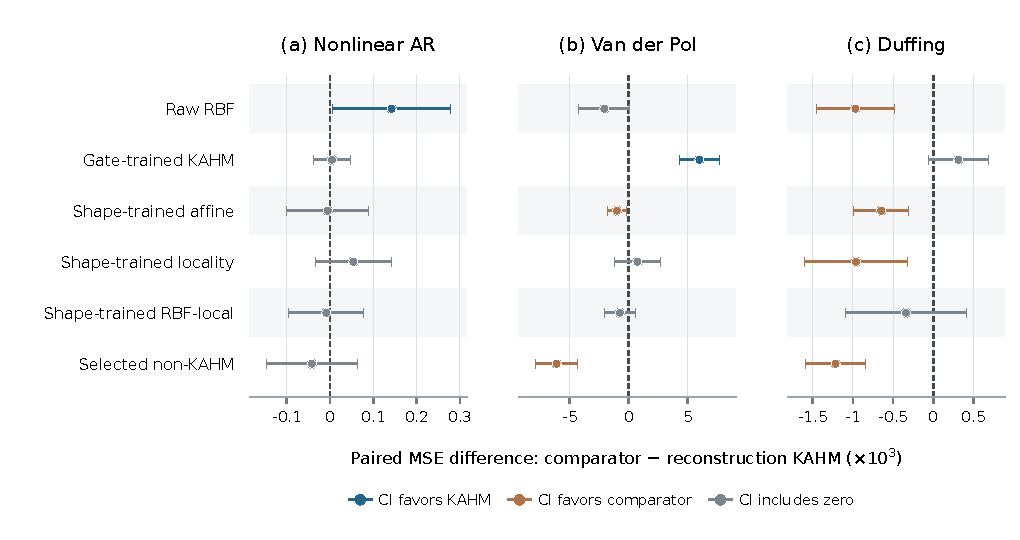
\includegraphics[width=\linewidth]{generated/direct_reconstruction/primary_contrasts.pdf}
\caption{All 18 primary direct-reconstruction contrasts. Points and
intervals show comparator-minus-KAHM MSE multiplied by 1,000. Blue
intervals favor KAHM, orange intervals favor the comparator, and gray
intervals contain zero. Two-sided Bonferroni-adjusted Student intervals
use twelve paired repetitions per law and 11 degrees of freedom.
Panel scales differ.}
\label{fig:direct-primary}
\end{figure}

On the available natural collections, KAHM has scaled MSE $0.371935$,
compared with $0.385625$ for ridge, a 3.55\% reduction. Raw RBF
($0.363007$), boosting ($0.352201$), and shape-trained RBF-local
($0.363835$) are more accurate. The ridge gain is concentrated in
Dominick; excluding that collection leaves a 0.00229\% improvement
across the other two collections. Twelve of the 21 available natural
horizons select zero KAHM correction, including every Sunspot horizon.
Table~\ref{tab:direct-natural} reports all collection-specific results.

The \DirectOptimizations{} geometry fits use
\DirectObjectiveEvaluations{} objective evaluations. Of these fits,
2,491 report convergence, 604 reach their evaluation budget, and one
has an abnormal optimizer stop; each retains its best finite candidate.
Mean synthetic pipeline time is 10.725\,s for reconstruction-trained
KAHM, 0.914\,s for gate-trained KAHM, 0.0774\,s for fixed KAHM,
0.0172\,s for raw RBF, and 0.653\,s for boosting. On the seven
available natural tasks, KAHM averages 7.929\,s, compared with
0.0130\,s for raw RBF and 0.655\,s for boosting.
Table~\ref{tab:direct-cost} and Figure~\ref{fig:direct-natural-cost}
report the complete accuracy and resource comparison. These costs
include model fitting, selection, querying, and state serialization;
they do not measure online update latency.
